% Source: https://tex.stackexchange.com/a/635555/6880 

\documentclass[conference]{IEEEtran}
\IEEEoverridecommandlockouts
\usepackage{nccmath, mathtools}

\usepackage{tikz}
\usetikzlibrary{arrows.meta,
                positioning,
                quotes}

%---------------- Show page layout. Don't use in a real document!
\usepackage{showframe}
\renewcommand\ShowFrameLinethickness{0.15pt}
\renewcommand*\ShowFrameColor{\color{red}}
%---------------------------------------------------------------%
\usepackage{lipsum}% For dummy text. Don't use in a real document
\begin{document}
    \begin{figure*}
    \centering
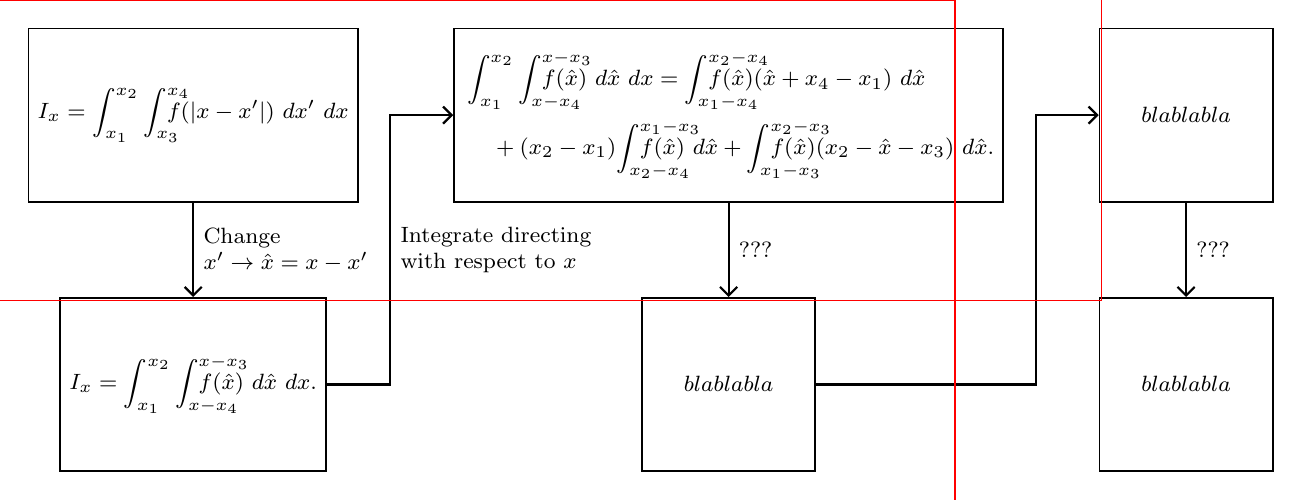
\begin{tikzpicture}[
node distance = 12mm and 12mm,
   arr/.style = {draw, -Straight Barb, thick},
   lbl/.style = {font=\footnotesize, align=left, pos=0.75, right},
     N/.style = {draw, semithick, minimum size=22mm},
every edge/.style = {arr},
every edge quotes/.style = {auto, font=\footnotesize, align=left}
                        ]
\node[N] (A)
{
$\medmath{I_{x} = \int_{x_1}^{x_2} 
                    \mathrlap{\int_{x_3}^{x_4}}
                    \quad f(|x-x'|)~dx'~dx}
$
};
\node[N] (B) [below=of A]  
{
$\medmath{I_{x} = \int_{x_1}^{x_2} 
                    \mathrlap{\int_{x-x_4}^{x-x_3}}
                        \quad f(\hat{x})~ d\hat{x}~dx.}
$
};

\node[N] (C) [right=of A] 
{
$\medmath{\begin{multlined}%\label{eq:int_p_single_case1a}
\int_{x_1}^{x_2}
\mathrlap{\int_{x-x_4}^{x-x_3}}
    \quad f(\hat{x}) ~d\hat{x}~dx 
 = \mathrlap{\int_{x_1-x_4}^{x_2-x_4} }
    \quad f(\hat{x}) (\hat{x} + x_4 - x_1)~ d\hat{x}    \\ 
    {} + (x_2 - x_1) 
        \mathrlap{\int_{x_2-x_4}^{x_1-x_3}}
        \quad f(\hat{x}) ~d\hat{x} +
        \mathrlap{\int_{x_1-x_3}^{x_2-x_3}}
        \quad f(\hat{x})(x_2 - \hat{x} - x_3)~d\hat{x} .
    \end{multlined}}
$
};

\node[N] (D) [below=of C] {$\medmath{blablabla}$};
\node[N] (E) [right=of C] {$\medmath{blablabla}$};
\node[N] (F) [below=of E] {$\medmath{blablabla}$};
%%%% arrows
\path   (A) edge["Change\\ $x'\to\hat{x} = x - x'$"] (B)
        (C) edge["???"] (D)
        (E) edge["???"] (F);
\coordinate[left=8mm of C.west] (aux1);
\coordinate[left=8mm of E.west] (aux2);
\draw[arr]  (B) -| (aux1) node[lbl] {Integrate directing\\ 
                                    with respect to $x$}
                -- (C);
\draw[arr]  (D) -| (aux2)
                |- (E);

\end{tikzpicture}
\end{figure*}
\end{document}